\documentclass{standalone}
\usepackage{tikz}
\usetikzlibrary{patterns, positioning}

\begin{document}
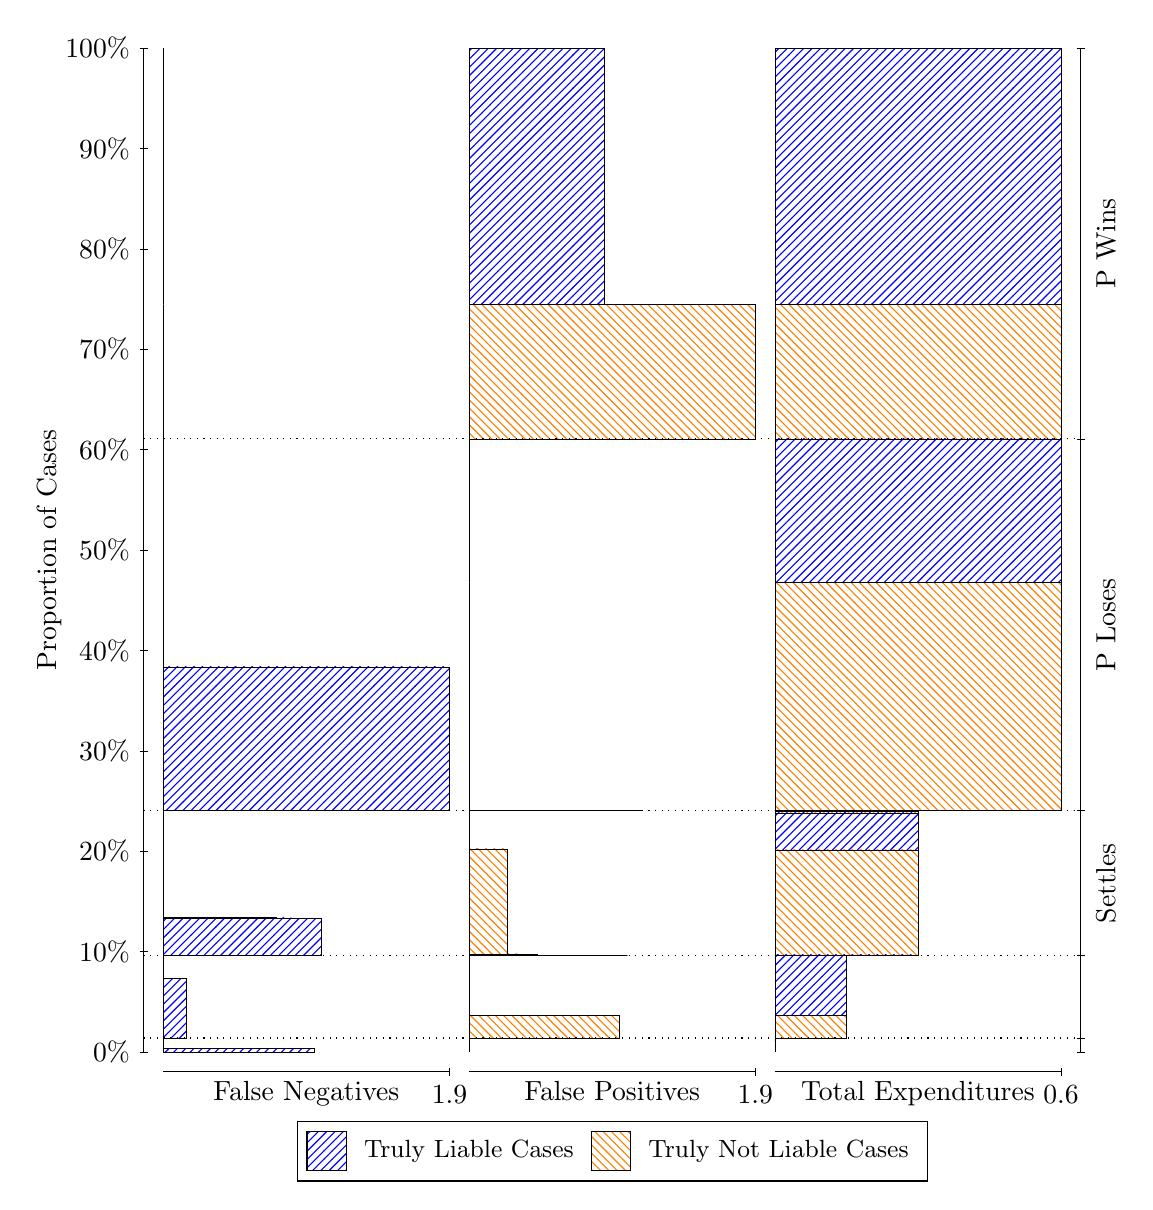
\begin{tikzpicture}
\draw[black, very thin] (1.5,1.75) -- (1.5,14.5);
\node[rotate=90, anchor=center] at (0.3, 8.125) {Proportion of Cases};
\draw[black, very thin] (1.45,1.75) -- (1.55,1.75);
\node[anchor=east] at (1.45, 1.75) {0\%};
\draw[black, very thin] (1.45,3.025) -- (1.55,3.025);
\node[anchor=east] at (1.45, 3.025) {10\%};
\draw[black, very thin] (1.45,4.3) -- (1.55,4.3);
\node[anchor=east] at (1.45, 4.3) {20\%};
\draw[black, very thin] (1.45,5.575) -- (1.55,5.575);
\node[anchor=east] at (1.45, 5.575) {30\%};
\draw[black, very thin] (1.45,6.85) -- (1.55,6.85);
\node[anchor=east] at (1.45, 6.85) {40\%};
\draw[black, very thin] (1.45,8.125) -- (1.55,8.125);
\node[anchor=east] at (1.45, 8.125) {50\%};
\draw[black, very thin] (1.45,9.4) -- (1.55,9.4);
\node[anchor=east] at (1.45, 9.4) {60\%};
\draw[black, very thin] (1.45,10.675) -- (1.55,10.675);
\node[anchor=east] at (1.45, 10.675) {70\%};
\draw[black, very thin] (1.45,11.95) -- (1.55,11.95);
\node[anchor=east] at (1.45, 11.95) {80\%};
\draw[black, very thin] (1.45,13.225) -- (1.55,13.225);
\node[anchor=east] at (1.45, 13.225) {90\%};
\draw[black, very thin] (1.45,14.5) -- (1.55,14.5);
\node[anchor=east] at (1.45, 14.5) {100\%};

\draw[black, very thin] (13.4,1.75) -- (13.4,14.5);
\draw[black, very thin] (13.35,1.75) -- (13.45,1.75);
\node[anchor=west] at (13.35, 1.75) {};
\draw[black, very thin] (13.35,1.9273) -- (13.45,1.9273);
\node[anchor=west] at (13.35, 1.9273) {};
\draw[black, very thin] (13.35,2.973) -- (13.45,2.973);
\node[anchor=west] at (13.35, 2.973) {};
\draw[black, very thin] (13.35,4.8148) -- (13.45,4.8148);
\node[anchor=west] at (13.35, 4.8148) {};
\draw[black, very thin] (13.35,4.8148) -- (13.45,4.8148);
\node[anchor=west] at (13.35, 4.8148) {};
\draw[black, very thin] (13.35,9.5364) -- (13.45,9.5364);
\node[anchor=west] at (13.35, 9.5364) {};
\draw[black, very thin] (13.35,14.5) -- (13.45,14.5);
\node[anchor=west] at (13.35, 14.5) {};

\draw[black, very thin, pattern color=blue, pattern=north east lines] (1.75,1.75) rectangle (3.6623,1.7987);
\draw[black, very thin, pattern color=orange, pattern=north west lines] (1.75,1.7987) rectangle (1.75,1.9273);
\draw[black, very thin, pattern color=blue, pattern=north east lines] (1.75,1.9273) rectangle (2.0368,2.6881);
\draw[black, very thin, pattern color=orange, pattern=north west lines] (1.75,2.6881) rectangle (1.75,2.973);
\draw[black, very thin, pattern color=blue, pattern=north east lines] (1.75,2.973) rectangle (3.7579,3.4417);
\draw[black, very thin, pattern color=blue, pattern=north east lines] (1.75,3.4417) rectangle (3.5667,3.4424);
\draw[black, very thin, pattern color=blue, pattern=north east lines] (1.75,3.4424) rectangle (3.3754,3.453);
\draw[black, very thin, pattern color=blue, pattern=north east lines] (1.75,3.453) rectangle (3.1842,3.4544);
\draw[black, very thin, pattern color=blue, pattern=north east lines] (1.75,3.4544) rectangle (2.993,3.4593);
\draw[black, very thin, pattern color=blue, pattern=north east lines] (1.75,3.4593) rectangle (2.8018,3.4593);
\draw[black, very thin, pattern color=blue, pattern=north east lines] (1.75,3.4593) rectangle (2.6105,3.4593);
\draw[black, very thin, pattern color=blue, pattern=north east lines] (1.75,3.4593) rectangle (2.4193,3.4593);
\draw[black, very thin, pattern color=blue, pattern=north east lines] (1.75,3.4593) rectangle (2.2281,3.4593);
\draw[black, very thin, pattern color=orange, pattern=north west lines] (1.75,3.4593) rectangle (1.75,4.8148);
\draw[black, very thin, pattern color=blue, pattern=north east lines] (1.75,4.8148) rectangle (2.0368,4.8148);
\draw[black, very thin, pattern color=orange, pattern=north west lines] (1.75,4.8148) rectangle (1.75,4.8148);
\draw[black, very thin, pattern color=blue, pattern=north east lines] (1.75,4.8148) rectangle (5.3833,6.6402);
\draw[black, very thin, pattern color=orange, pattern=north west lines] (1.75,6.6402) rectangle (1.75,9.5364);
\draw[black, very thin, pattern color=orange, pattern=north west lines] (1.75,9.5364) rectangle (1.75,11.246);
\draw[black, very thin, pattern color=blue, pattern=north east lines] (1.75,11.246) rectangle (1.75,14.5);
\draw[black, very thin, pattern color=orange, pattern=north west lines] (5.6333,1.75) rectangle (5.6333,1.8787);
\draw[black, very thin, pattern color=blue, pattern=north east lines] (5.6333,1.8787) rectangle (5.6333,1.9273);
\draw[black, very thin, pattern color=orange, pattern=north west lines] (5.6333,1.9273) rectangle (7.5456,2.2123);
\draw[black, very thin, pattern color=blue, pattern=north east lines] (5.6333,2.2123) rectangle (5.6333,2.973);
\draw[black, very thin, pattern color=orange, pattern=north west lines] (5.6333,2.973) rectangle (7.6412,2.973);
\draw[black, very thin, pattern color=orange, pattern=north west lines] (5.6333,2.973) rectangle (7.45,2.973);
\draw[black, very thin, pattern color=orange, pattern=north west lines] (5.6333,2.973) rectangle (7.2588,2.973);
\draw[black, very thin, pattern color=orange, pattern=north west lines] (5.6333,2.973) rectangle (7.0675,2.973);
\draw[black, very thin, pattern color=orange, pattern=north west lines] (5.6333,2.973) rectangle (6.8763,2.9765);
\draw[black, very thin, pattern color=orange, pattern=north west lines] (5.6333,2.9765) rectangle (6.6851,2.9772);
\draw[black, very thin, pattern color=orange, pattern=north west lines] (5.6333,2.9772) rectangle (6.6851,2.9772);
\draw[black, very thin, pattern color=orange, pattern=north west lines] (5.6333,2.9772) rectangle (6.4939,2.9923);
\draw[black, very thin, pattern color=orange, pattern=north west lines] (5.6333,2.9923) rectangle (6.3026,2.9947);
\draw[black, very thin, pattern color=orange, pattern=north west lines] (5.6333,2.9947) rectangle (6.1114,4.3286);
\draw[black, very thin, pattern color=blue, pattern=north east lines] (5.6333,4.3286) rectangle (5.7289,4.3286);
\draw[black, very thin, pattern color=blue, pattern=north east lines] (5.6333,4.3286) rectangle (5.6333,4.8148);
\draw[black, very thin, pattern color=orange, pattern=north west lines] (5.6333,4.8148) rectangle (7.8325,4.8148);
\draw[black, very thin, pattern color=blue, pattern=north east lines] (5.6333,4.8148) rectangle (5.9202,4.8148);
\draw[black, very thin, pattern color=orange, pattern=north west lines] (5.6333,4.8148) rectangle (5.6333,7.711);
\draw[black, very thin, pattern color=blue, pattern=north east lines] (5.6333,7.711) rectangle (5.6333,9.5364);
\draw[black, very thin, pattern color=orange, pattern=north west lines] (5.6333,9.5364) rectangle (9.2667,11.246);
\draw[black, very thin, pattern color=blue, pattern=north east lines] (5.6333,11.246) rectangle (7.3544,14.5);
\draw[black, very thin, pattern color=orange, pattern=north west lines] (9.5167,1.75) rectangle (9.5167,1.8787);
\draw[black, very thin, pattern color=blue, pattern=north east lines] (9.5167,1.8787) rectangle (9.5167,1.9273);
\draw[black, very thin, pattern color=orange, pattern=north west lines] (9.5167,1.9273) rectangle (10.425,2.2123);
\draw[black, very thin, pattern color=blue, pattern=north east lines] (9.5167,2.2123) rectangle (10.425,2.973);
\draw[black, very thin, pattern color=orange, pattern=north west lines] (9.5167,2.973) rectangle (11.333,2.9772);
\draw[black, very thin, pattern color=blue, pattern=north east lines] (9.5167,2.9772) rectangle (11.333,2.9835);
\draw[black, very thin, pattern color=orange, pattern=north west lines] (9.5167,2.9835) rectangle (11.333,4.3174);
\draw[black, very thin, pattern color=blue, pattern=north east lines] (9.5167,4.3174) rectangle (11.333,4.786);
\draw[black, very thin, pattern color=orange, pattern=north west lines] (9.5167,4.786) rectangle (11.333,4.8035);
\draw[black, very thin, pattern color=blue, pattern=north east lines] (9.5167,4.8035) rectangle (11.333,4.8148);
\draw[black, very thin, pattern color=orange, pattern=north west lines] (9.5167,4.8148) rectangle (11.333,4.8148);
\draw[black, very thin, pattern color=blue, pattern=north east lines] (9.5167,4.8148) rectangle (11.333,4.8148);
\draw[black, very thin, pattern color=orange, pattern=north west lines] (9.5167,4.8148) rectangle (13.15,7.711);
\draw[black, very thin, pattern color=blue, pattern=north east lines] (9.5167,7.711) rectangle (13.15,9.5364);
\draw[black, very thin, pattern color=orange, pattern=north west lines] (9.5167,9.5364) rectangle (13.15,11.246);
\draw[black, very thin, pattern color=blue, pattern=north east lines] (9.5167,11.246) rectangle (13.15,14.5);
\draw[black, dotted] (1.5,1.9273) -- (13.4,1.9273);
\draw[black, dotted] (1.5,2.973) -- (13.4,2.973);
\draw[black, dotted] (1.5,4.8148) -- (13.4,4.8148);
\draw[black, dotted] (1.5,4.8148) -- (13.4,4.8148);
\draw[black, dotted] (1.5,9.5364) -- (13.4,9.5364);
\draw[black, very thin] (1.75,1.5) -- (5.3833,1.5);
\node[anchor=north] at (3.5667, 1.5) {False Negatives};
\draw[black, very thin] (5.3833,1.45) -- (5.3833,1.55);
\node[anchor=north] at (5.3833, 1.45) {1.9};

\draw[black, very thin] (5.6333,1.5) -- (9.2667,1.5);
\node[anchor=north] at (7.45, 1.5) {False Positives};
\draw[black, very thin] (9.2667,1.45) -- (9.2667,1.55);
\node[anchor=north] at (9.2667, 1.45) {1.9};

\draw[black, very thin] (9.5167,1.5) -- (13.15,1.5);
\node[anchor=north] at (11.333, 1.5) {Total Expenditures};
\draw[black, very thin] (13.15,1.45) -- (13.15,1.55);
\node[anchor=north] at (13.15, 1.45) {0.6};



\node[black, centered, rotate=90] at (13.72, 3.8939) {Settles};

\node[black, centered, rotate=90] at (13.72, 7.1756) {P Loses};
\node[black, centered, rotate=90] at (13.72, 12.018) {P Wins};

\draw (7.449999999999999,1.5) node[draw=none] (baseCoordinate) {};
\begin{scope}[align=center]
        \matrix[scale=0.5, draw=black, below=0.5cm of baseCoordinate, nodes={draw}, column sep=0.1cm]{
            \node[rectangle, draw, minimum width=0.5cm, minimum height=0.5cm, pattern=north east lines, pattern color=blue] {}; &
            \node[draw=none, font=\small] (B) {Truly Liable Cases}; &
            \node[rectangle, draw, minimum width=0.5cm, minimum height=0.5cm, pattern=north west lines, pattern color=orange] {}; &
            \node[draw=none, font=\small] (B) {Truly Not Liable Cases}; \\
            };
\end{scope}

\end{tikzpicture}
\end{document}